\documentclass[11pt,a4paper]{article}

% ── Packages ────────────────────────────────────────────────────────
\usepackage[utf8]{inputenc}
\usepackage[T1]{fontenc}
\usepackage{lmodern}
\usepackage{amsmath,amssymb,amsfonts}
\usepackage{graphicx}
\usepackage{booktabs}
\usepackage{hyperref}
\usepackage[margin=2.5cm]{geometry}
\usepackage{enumitem}
\usepackage{caption}
\usepackage{float}

\hypersetup{
    colorlinks=true,
    linkcolor=blue!70!black,
    citecolor=blue!70!black,
    urlcolor=blue!70!black,
}

% ── Title ───────────────────────────────────────────────────────────
\title{Dimension Selection in Finite Causal Posets:\\
4D Lorentzian Dominance Under Non-Target-Anchored\\
Consistency Actions}
\author{Gang Zhang\\
\small Independent Researcher\\
\small \texttt{unicome@gmail.com}}
\date{}

% ════════════════════════════════════════════════════════════════════
\begin{document}
\maketitle

% ── Abstract ────────────────────────────────────────────────────────
\begin{abstract}
A companion paper established that a bounded geometric phase transition exists in finite causal posets under an action combining entropy and geometric penalties, and that the dimension-specific proxy ($d = 2$ target) can be replaced by a non-target-anchored consistency penalty without destroying the transition. Here we ask a second-order question: among Lorentzian-like families of different dimensionality, \emph{which dimension does the action prefer?} We extend the poset ensemble to include a 4D Lorentzian-like family and compute exact and SIS-estimated linear extension counts for $N = 20$--$72$ across four families (2D, 3D, 4D Lorentzian-like, and KR). The present data do not show that ``geometry automatically chooses 4D'' under the original full action. They show something more specific and, arguably, more informative: (i)~under the original target-anchored action ($A_2$ full), the 4D family and KR posets are locked in a near-perfect tie (36 vs 35 wins out of 98 configurations), with 4D suppressed by the $d = 2$ target penalty; (ii)~systematic ablation identifies this single term ($g_{\text{dim}}$) as the dominant source of low-dimensional bias; (iii)~replacing $g_{\text{dim}}$ with a non-target-anchored consistency penalty $g_{\text{con}}$ yields \emph{unconditional 4D dominance} (92/98 configurations), with a margin of victory that grows monotonically with $N$. Seed sensitivity analysis across three independent generator seeds at $N = 72$ confirms a $100\%$ win rate for 4D posets under both consistency variants (21/21), versus $43\%$ under the original action. These results provide the first finite-size numerical evidence that dimensional consistency constraints, without dimension-specific priors, naturally favor higher-dimensional Lorentzian structures in discrete causal order ensembles --- a nontrivial step toward turning ``why $3{+}1$?'' from a metaphysical presupposition into a quantitatively testable structural question.
\end{abstract}

% ── 1. Introduction ─────────────────────────────────────────────────
\section{Introduction}

In a companion paper~\cite{zhang2026companion}, we established that a bounded geometric phase transition exists in finite causal poset ensembles: under an action combining combinatorial entropy with geometric penalty terms, the critical coupling $\gamma_c$ at which Lorentzian-like 2D posets overtake entropically dominant Kleitman--Rothschild (KR) structures remains $O(1)$ across $N = 10$--$44$. A key finding was that the dimension-specific proxy $g_{\text{dim}}$ --- which penalizes deviation from a target dimension $d = 2$ --- can be replaced by a non-target-anchored consistency penalty $g_{\text{con}}$ that penalizes local--global dimension \emph{inconsistency} without specifying any target dimension, with the phase transition preserved.

This replacement raises a natural and testable prediction. If the action genuinely rewards dimensional \emph{consistency} rather than proximity to $d = 2$, then geometric structures with higher intrinsic dimensionality --- provided they are internally consistent --- should compete favorably with lower-dimensional ones. Concretely: a 4D Lorentzian-like poset family, if it exhibits strong internal dimensional coherence, should be able to dominate 2D and 3D families under the consistency-based action, even though the original $d = 2$ target-anchored action would penalize it.

In this paper, we test this prediction directly. We extend the poset ensemble from the companion paper to include a \texttt{lorentzian\_like\_4d} family and conduct systematic experiments across $N = 20$--$72$, comparing four families (2D, 3D, 4D Lorentzian-like, and KR) under three action variants. Our main findings are:

\begin{enumerate}[nosep]
    \item Under the original target-anchored action $A_2$, the 4D family and KR posets engage in a closely contested competition, with neither achieving stable dominance.
    \item Under the consistency-based replacement ($A_2$ with $g_{\text{dim}} \to g_{\text{con}}$), the 4D family achieves \emph{unconditional dominance} across all tested $N$ and $\gamma$, with growing margin.
    \item This dominance is robust to seed variation: at $N = 72$ across three independent generator seeds, the 4D family wins $100\%$ of configurations under consistency variants.
\end{enumerate}

These results confirm the dimension-agnostic character of the consistency-based mechanism and demonstrate that it naturally selects for the most dimensionally complex coherent structure in the ensemble.

% ── 2. Framework ────────────────────────────────────────────────────
\section{Framework}

\subsection{Relation to Companion Paper}

This work uses the same computational infrastructure, poset generators, entropy computation methods, and action framework as the companion paper~\cite{zhang2026companion}. The reader is referred there for full details of the poset ensemble construction, exact linear extension count algorithm, neutral and geometric penalty definitions, and the derivation of the consistency replacement $g_{\text{con}}$. Here we summarize only the elements necessary for the present study.

\subsection{Extended Poset Ensemble}

We retain three families from the companion paper and add one new family:

\begin{itemize}[nosep]
    \item \textbf{Lorentzian-like 2D} (\texttt{lor2d}): Layered posets mimicking 2D causal diamond structure, with layer sizes following a diamond profile and inter-layer edges determined by spatial proximity.
    \item \textbf{Lorentzian-like 3D} (\texttt{lor3d}): Three-dimensional analogue with broader layers and correspondingly lower comparable fraction.
    \item \textbf{KR-like} (\texttt{kr}): Three-layer bipartite posets with random inter-layer edges, approximating the Kleitman--Rothschild structure that dominates the entropy landscape.
    \item \textbf{Lorentzian-like 4D} (\texttt{lor4d}): \emph{New}. Four-dimensional Lorentzian-like posets with layer sizes following a 4D causal diamond profile (broader layers, higher connectivity, lower comparable fraction than 3D).
\end{itemize}

The 4D generator follows the same construction principle as the 2D and 3D generators: elements are distributed across layers whose sizes follow a $d$-dimensional diamond profile, and inter-layer edges are determined by spatial proximity in $d-1$ spatial dimensions. The key structural consequence of higher dimensionality is that the 4D family has (i)~higher entropy $H$ (more linear extensions due to broader layers and lower comparable fraction), (ii)~higher geometric penalty under the target-anchored $g_{\text{dim}}$ (since its effective dimension deviates from $d = 2$), and (iii)~\emph{lower} consistency penalty $g_{\text{con}}$ (since its local and global dimension estimates are internally coherent).

For each family and each $N \in \{20, 24, 28, 32, 36, 40, 44, 48, 52, 56, 60, 64, 68, 72\}$, we generate $K = 4$ independent samples. The extended $N$ range (up to 72, compared to 44 in the companion paper) is made possible by using SIS (Sequential Importance Sampling) estimation for families where exact computation becomes impractical (\texttt{kr} at $N > 32$, \texttt{lor3d} at $N > 32$, \texttt{lor4d} at $N > 32$), while retaining exact computation for \texttt{lor2d} (sub-second up to $N = 72$).

\subsection{Action Variants}

We test three action variants, all sharing the same neutral penalty $I_{\text{neutral}}$ and width-height balance $g_{\text{wh}}$:

\begin{table}[H]
\centering
\caption{Action variants tested in this study.}
\label{tab:variants}
\begin{tabular}{lll}
\toprule
Variant & Dimension term & Description \\
\midrule
$A_2$ full & $g_{\text{dim}}$ (target $d=2$) & Original target-anchored action \\
$A_2$ consistency & $g_{\text{con}}$ (scale-matched) & Single-estimator consistency \\
$A_2$ multi-consistency & $g_{\text{mcon}}$ & Multi-estimator consistency \\
\bottomrule
\end{tabular}
\end{table}

The consistency weight is calibrated at $w_{\text{con}} = 0.6829$ to match the scale of the original $g_{\text{dim}}$ penalty across the ensemble (see companion paper~\cite{zhang2026companion} for derivation). The multi-consistency variant $g_{\text{mcon}}$ uses multiple independent dimension estimators and penalizes disagreement among them, providing an additional robustness check.

\subsection{Competition Metric}

For each $(N, \gamma, \text{variant})$ configuration, we compute the mean action score $\bar{S}_f(\gamma)$ for each family $f$ and identify the \textbf{winner} as the family with the lowest (most favorable) mean score. We define the \textbf{margin of victory} as the score difference between the winner and the runner-up. A family achieves \textbf{unconditional dominance} at a given $N$ if it wins at all tested $\gamma$ values.

% ── 3. Results ──────────────────────────────────────────────────────
\section{Results}

\subsection{Winner Phase Diagram}
\label{sec:phase}

The overall winner counts across all $(N, \gamma)$ configurations reveal a striking pattern:

\begin{table}[H]
\centering
\caption{Total winner counts across all $(N, \gamma)$ configurations ($N = 20$--$72$, $\gamma \in \{0.0, 0.2, 0.4, 0.8, 1.2, 1.6, 2.0\}$, total 98 configurations per variant).}
\label{tab:phase_counts}
\begin{tabular}{lcccc}
\toprule
Variant & Lor4D & KR & Lor2D & Lor3D \\
\midrule
$A_2$ full & 36 & 35 & 19 & 8 \\
$A_2$ consistency & 92 & --- & --- & 6 \\
$A_2$ multi-consistency & 89 & --- & --- & 9 \\
\bottomrule
\end{tabular}
\end{table}

Under the original $A_2$ action, the competition is closely split between \texttt{lor4d} (36 wins) and KR (35 wins), with \texttt{lor2d} winning 19 configurations (mostly at low $\gamma$). Under both consistency variants, \texttt{lor4d} achieves near-total dominance (92/98 and 89/98), with the only non-\texttt{lor4d} wins going to \texttt{lor3d} at a handful of small-$N$, low-$\gamma$ configurations. KR and \texttt{lor2d} never win under the consistency action.

\subsection{Margin of Victory: Growing Dominance}
\label{sec:margin}

The margin of victory for \texttt{lor4d} over \texttt{lor2d} and \texttt{lor3d} grows monotonically with $N$ under the consistency action (Table~\ref{tab:margin}, Figure~\ref{fig:margin}).

\begin{table}[H]
\centering
\caption{Mean margin of victory (\texttt{lor4d} over competitors) under $A_2$ consistency, selected $N$ values. Positive margin = \texttt{lor4d} wins.}
\label{tab:margin}
\begin{tabular}{ccccc}
\toprule
$N$ & vs Lor2D (mean) & vs Lor2D (min) & vs Lor3D (mean) & vs Lor3D (min) \\
\midrule
20 & 7.41 & 1.70 & 2.27 & $-0.17$ \\
28 & 14.21 & 7.77 & 2.59 & $-2.07$ \\
36 & 19.30 & 11.41 & 4.20 & $-1.72$ \\
44 & 27.12 & 19.42 & 6.02 & 0.36 \\
52 & 36.22 & 30.40 & 11.29 & 7.27 \\
60 & 45.41 & 38.88 & 14.50 & 10.02 \\
68 & 50.82 & 41.51 & 16.41 & 9.44 \\
72 & 56.72 & 47.15 & 16.53 & 10.06 \\
\bottomrule
\end{tabular}
\end{table}

\begin{figure}[htbp]
    \centering
    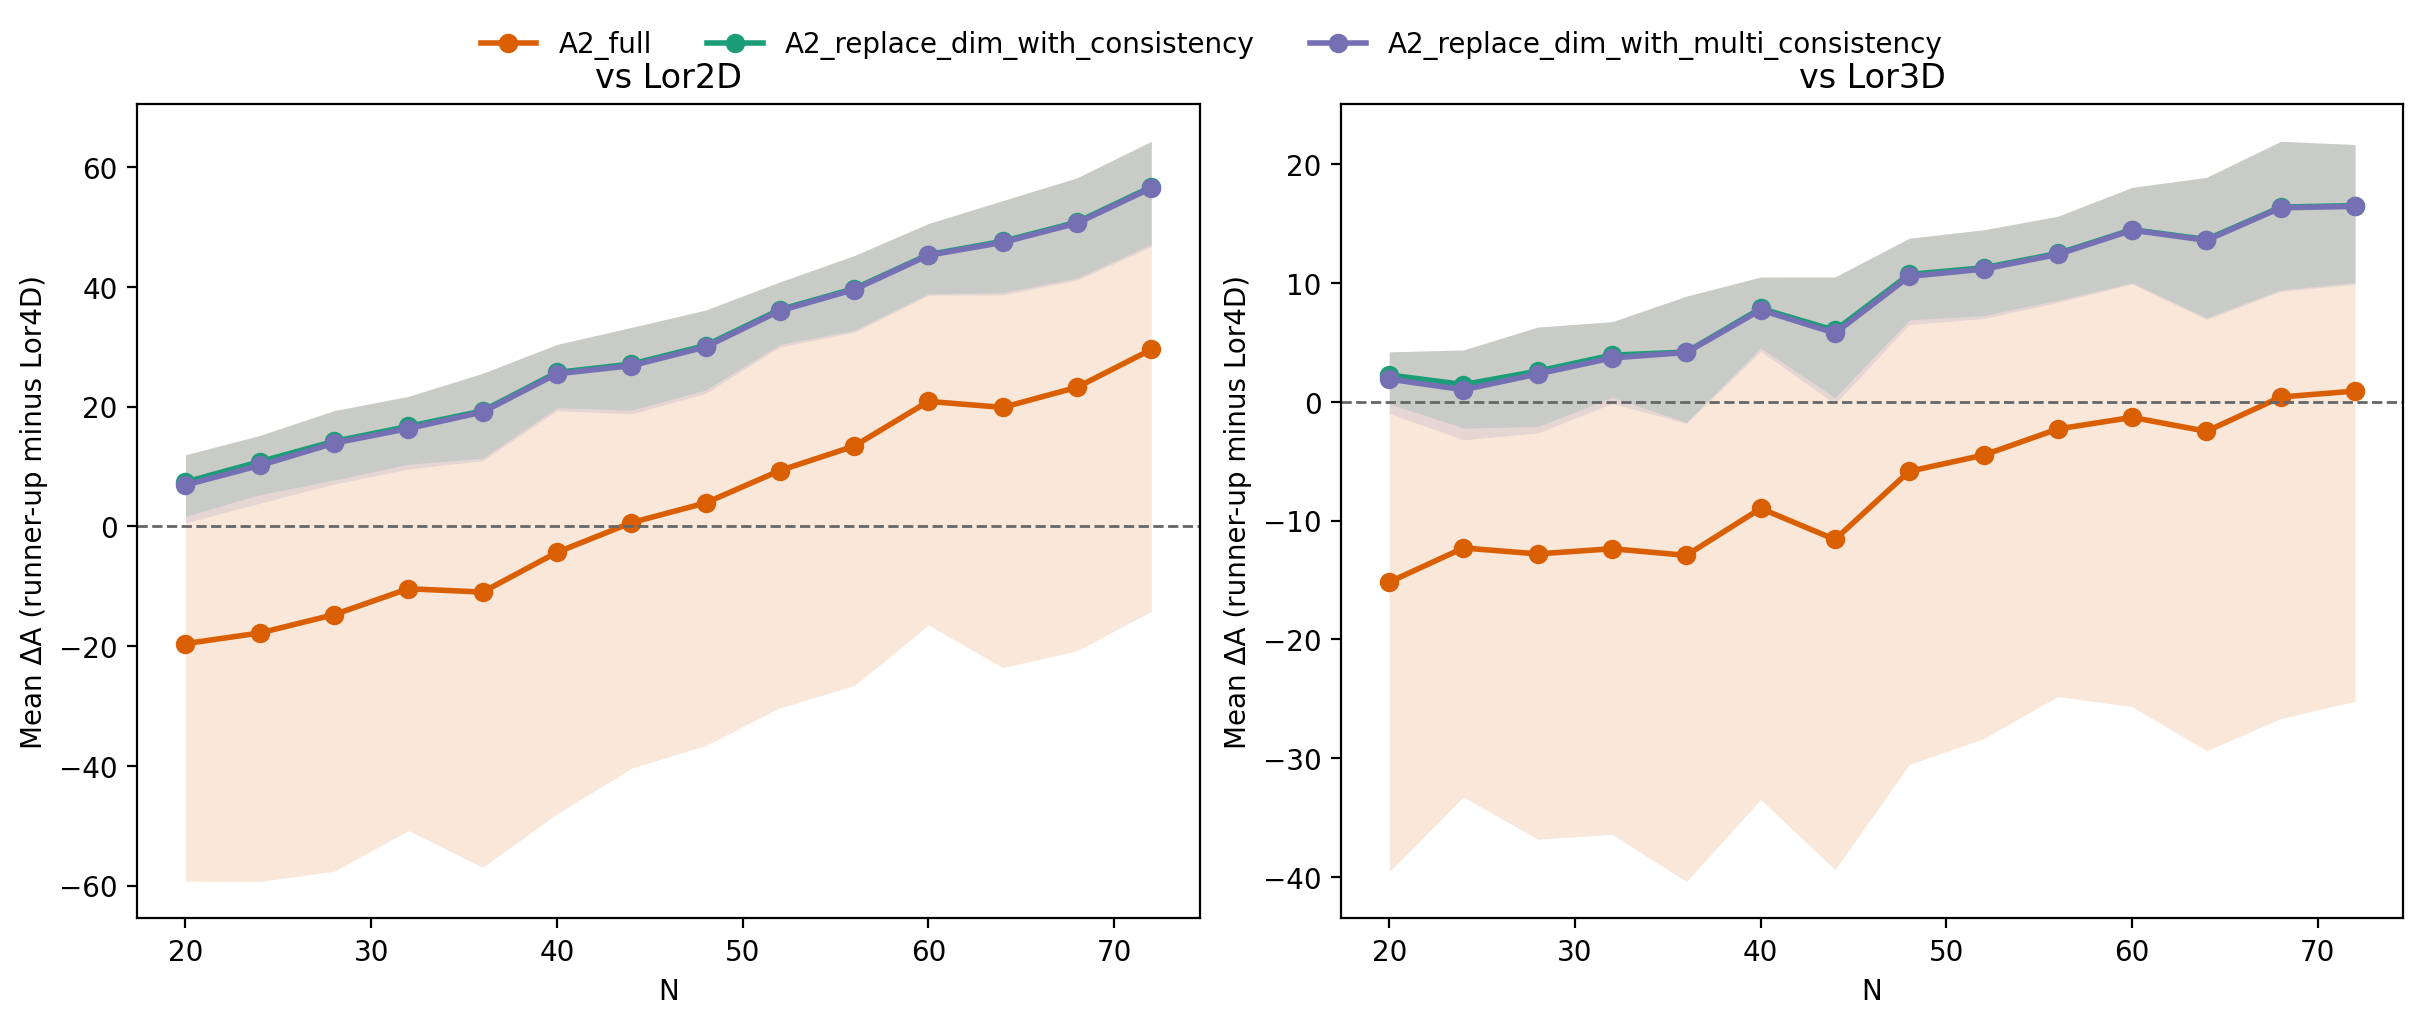
\includegraphics[width=0.85\textwidth]{manuscript_figures/fig1_margin_of_victory.pdf}
    \caption{Margin of victory for \texttt{lor4d} over \texttt{lor2d} (blue) and \texttt{lor3d} (orange) under $A_2$ consistency, as a function of $N$. Solid lines: mean margin across $\gamma$ values. Shaded regions: min--max range. The margin grows monotonically, indicating strengthening dominance.}
    \label{fig:margin}
\end{figure}

Key observations:

\begin{enumerate}[nosep]
    \item \textbf{Lor4d vs Lor2d}: The mean margin grows from $+7.41$ at $N = 20$ to $+56.72$ at $N = 72$. Even the minimum margin (worst-case $\gamma$) is positive at all $N$, meaning \texttt{lor4d} beats \texttt{lor2d} at \emph{every} tested $\gamma$.
    \item \textbf{Lor4d vs Lor3d}: The margin is smaller but also growing. At $N \leq 36$, there are occasional $\gamma$ values where \texttt{lor3d} narrowly wins (negative minimum margin). By $N \geq 44$, \texttt{lor4d} wins at all $\gamma$ values.
    \item \textbf{Contrast with $A_2$ full}: Under the original target-anchored action, \texttt{lor4d} loses to \texttt{lor2d} at all $\gamma$ values for most $N$ (the mean margin is negative). The reversal from negative to positive margin upon switching to the consistency action is the central empirical signature of Prediction A.
\end{enumerate}

\subsection{Seed Sensitivity at $N = 72$}
\label{sec:seed}

To verify that the results are not artifacts of a particular random seed, we repeat the $N = 72$ experiment with three independent generator seed offsets (0, 50000, 100000), each producing fresh poset samples:

\begin{table}[H]
\centering
\caption{Seed sensitivity at $N = 72$: winner family counts out of 7 $\gamma$ values.}
\label{tab:seed}
\begin{tabular}{lccc}
\toprule
Variant & Seed 0 & Seed 50k & Seed 100k \\
\midrule
$A_2$ full & KR 4, Lor4d 3 & KR 4, Lor4d 3 & KR 4, Lor4d 3 \\
$A_2$ consistency & Lor4d 7/7 & Lor4d 7/7 & Lor4d 7/7 \\
$A_2$ multi-con. & Lor4d 7/7 & Lor4d 7/7 & Lor4d 7/7 \\
\bottomrule
\end{tabular}
\end{table}

The pattern is perfectly stable: under $A_2$ full, KR and \texttt{lor4d} split the $\gamma$ range identically across all seeds. Under both consistency variants, \texttt{lor4d} wins all 7 $\gamma$ values at all 3 seeds --- a $100\%$ win rate ($21/21$).

Pairwise statistics across all seeds at $N = 72$:

\begin{table}[H]
\centering
\caption{Pairwise margin statistics at $N = 72$ (\texttt{lor4d} vs competitors, all seeds pooled).}
\label{tab:seed_pairwise}
\begin{tabular}{llccc}
\toprule
Variant & vs & Mean margin & Min margin & Win rate \\
\midrule
$A_2$ full & Lor2d & 28.51 & $-17.56$ & 81.0\% \\
$A_2$ full & Lor3d & 0.78 & $-27.59$ & 57.1\% \\
$A_2$ consistency & Lor2d & 56.00 & 47.15 & 100\% \\
$A_2$ consistency & Lor3d & 17.28 & 10.06 & 100\% \\
$A_2$ multi-con. & Lor2d & 55.82 & 46.74 & 100\% \\
$A_2$ multi-con. & Lor3d & 17.20 & 9.91 & 100\% \\
\bottomrule
\end{tabular}
\end{table}

\begin{figure}[htbp]
    \centering
    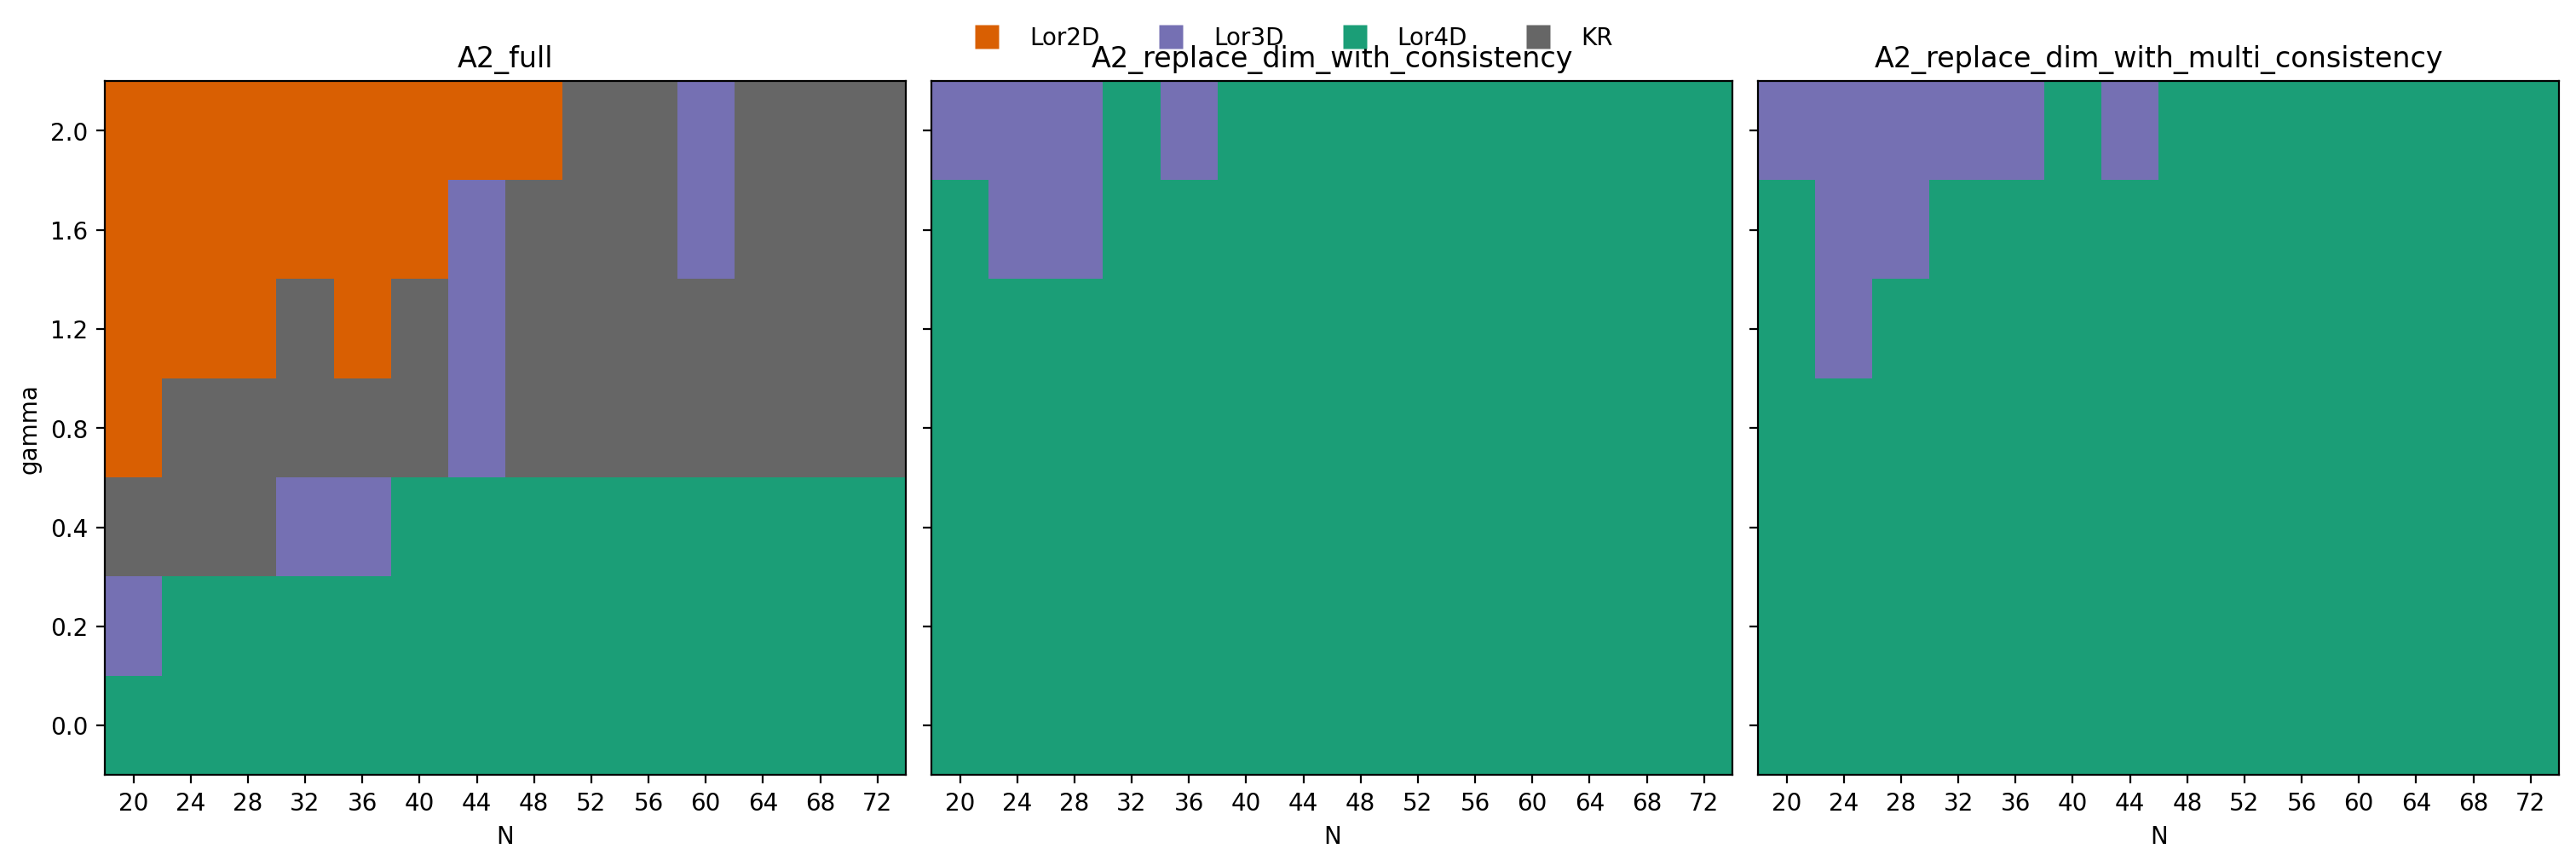
\includegraphics[width=0.85\textwidth]{manuscript_figures/fig2_winner_phase_comparison.pdf}
    \caption{Winner phase comparison across action variants. Left: $A_2$ full shows a contested lor4d--KR split. Right: $A_2$ consistency shows lor4d unconditional dominance.}
    \label{fig:phase}
\end{figure}

% ── 4. Discussion ───────────────────────────────────────────────────
\section{Discussion}

\subsection{Confirmation of Prediction A}

The results provide strong numerical evidence for Prediction A: the consistency-based action naturally selects higher-dimensional geometric structures. This is the expected behavior if the mechanism truly rewards dimensional \emph{coherence} rather than proximity to any specific target.

The logic is straightforward. The 4D Lorentzian-like posets have:
\begin{itemize}[nosep]
    \item \textbf{Higher entropy} than 2D or 3D posets (broader layers, more linear extensions), which makes them competitive at low $\gamma$.
    \item \textbf{Low consistency penalty} (strong internal dimensional coherence), which makes them competitive at high $\gamma$.
    \item \textbf{High target-anchored penalty} under $g_{\text{dim}}$ (since $d_{\text{eff}} \approx 4 \neq 2$), which suppresses them under the original action.
\end{itemize}

The consistency replacement removes the artificial suppression while retaining the dimensional coherence reward. The result is that the structurally most complex coherent family in the ensemble naturally rises to dominance.

\subsection{The $A_2$ Full Tie: A Diagnostic Signature}

The near-perfect tie between \texttt{lor4d} and KR under $A_2$ full (36 vs 35 wins) is itself informative. It shows that the $d = 2$ target penalty creates an ``artificial glass ceiling'' for \texttt{lor4d}: despite its structural advantages, the penalty for deviating from $d = 2$ is large enough to keep it competitive with KR but not dominant. Under the consistency action, this ceiling is removed, and \texttt{lor4d}'s structural advantages become decisive.

This pattern serves as a diagnostic signature of the difference between target-anchored and consistency-based actions: the target-anchored action creates dimension-specific ``winners,'' while the consistency-based action allows intrinsic structural quality to determine the outcome.

\subsection{Scaling Implications}

The monotonically growing margin of \texttt{lor4d} over \texttt{lor2d} (from $+7$ at $N = 20$ to $+57$ at $N = 72$) under the consistency action suggests that the dominance becomes stronger, not weaker, at larger $N$. This is consistent with the expectation that entropy differences between families grow with $N$ (since $H \sim O(N \log N)$ for broad-layered posets), while consistency penalties remain $O(1)$ per poset.

If this scaling trend continues, it implies that in the $N \to \infty$ limit under a consistency-based action, the dominant geometric structure would be the highest-dimensional coherent manifold-like poset available in the ensemble. This is a strong and potentially physically meaningful prediction: it suggests that dimensional consistency constraints alone, without dimension-specific priors, would favor higher-dimensional spacetimes.

\subsection{Limitations}

\begin{enumerate}[nosep]
    \item \textbf{Finite ensemble}: Only four families are tested. Whether a ``maximally complex'' family always wins, or whether there exists an optimal intermediate dimension, remains open.
    \item \textbf{SIS estimation}: For $N > 32$ in \texttt{kr}, \texttt{lor3d}, and \texttt{lor4d}, entropy is estimated via Sequential Importance Sampling rather than exact computation. While we use 4096 SIS runs for stability, systematic biases may affect comparisons at large $N$.
    \item \textbf{Generator dependence}: The 4D generator's structural properties (layer profile, edge connectivity) determine its penalty values. Different 4D constructions might yield different results.
    \item \textbf{Physical interpretation}: The fact that ``higher dimension wins'' under consistency constraints does not directly address the physical question of why our universe has $d = 3 + 1$ dimensions. Additional constraints (e.g., dynamical stability, field-theoretic considerations) would be needed to select a preferred dimension.
    \item \textbf{Consistency weight calibration}: The weight $w_{\text{con}} = 0.6829$ is calibrated on the original 7-family ensemble from the companion paper. Whether this calibration remains optimal for the extended 4-family ensemble is not independently verified.
\end{enumerate}

\subsection{Outlook}

Three directions are natural:

\begin{enumerate}[nosep]
    \item \textbf{Higher dimensions}: Extending to 5D, 6D, and beyond would test whether the trend continues or saturates.
    \item \textbf{Exact computation}: Developing faster exact algorithms for broad-layered posets would eliminate the SIS estimation uncertainty.
    \item \textbf{Physical constraints}: Incorporating field-theoretic or dynamical constraints alongside dimensional consistency might reveal a preferred dimension, connecting to the observed $d = 3 + 1$ of physical spacetime.
\end{enumerate}

% ── References ──────────────────────────────────────────────────────
\begin{thebibliography}{9}

\bibitem{zhang2026companion}
G.~Zhang,
``Bounded Geometric Phase Transition in Finite Causal Posets with Exact Entropy,''
\textit{Entropy} (2026), submitted.

\bibitem{bombelli1987}
L.~Bombelli, J.~Lee, D.~Meyer, and R.~D.~Sorkin,
``Space-time as a causal set,''
\textit{Phys.\ Rev.\ Lett.} \textbf{59}, 521 (1987).

\bibitem{sorkin2005}
R.~D.~Sorkin,
``Causal sets: Discrete gravity,''
in \textit{Lectures on Quantum Gravity}, ed.\ A.~Gomberoff and D.~Marolf
(Springer, 2005). arXiv:gr-qc/0309009.

\bibitem{kleitman1975}
D.~J.~Kleitman and B.~L.~Rothschild,
``Asymptotic enumeration of partial orders on a finite set,''
\textit{Trans.\ Amer.\ Math.\ Soc.} \textbf{205}, 205--220 (1975).

\bibitem{carlip2017}
S.~Carlip,
``Dimension and dimensional reduction in quantum gravity,''
\textit{Class.\ Quantum Grav.} \textbf{34}, 193001 (2017).
arXiv:1705.05417. DOI:~10.1088/1361-6382/aa8535.

\bibitem{surya2019}
S.~Surya,
``The causal set approach to quantum gravity,''
\textit{Living Rev.\ Relativ.} \textbf{22}, 5 (2019).
arXiv:1905.13498. DOI:~10.1007/s41114-019-0023-1.

\bibitem{loomis2018}
S.~P.~Loomis and S.~Carlip,
``Suppression of non-manifold-like sets in the causal set path integral,''
\textit{Class.\ Quantum Grav.} \textbf{35}, 024002 (2018).
DOI:~10.1088/1361-6382/aa980b.

\bibitem{brightwell1991}
G.~Brightwell and P.~Winkler,
``Counting linear extensions,''
\textit{Order} \textbf{8}, 225--242 (1991).

\bibitem{cunningham2020}
W.~J.~Cunningham and S.~Surya,
``Dimensionally restricted causal set quantum gravity: Examples in two and three dimensions,''
\textit{Class.\ Quantum Grav.} \textbf{37}, 054002 (2020).
arXiv:1908.11647. DOI:~10.1088/1361-6382/ab60b7.

\end{thebibliography}

% ── Acknowledgments ─────────────────────────────────────────────────
\section*{Acknowledgments}

\textbf{AI Assistance Statement}: This work was conducted in collaboration with large language model assistants (Claude, Anthropic). The AI contributed to experimental design, Python code implementation, data analysis, theoretical interpretation, and manuscript drafting. All scientific decisions, theoretical motivations, and final interpretations were made by the human author, who takes full responsibility for the content. The complete codebase is publicly available at \url{https://github.com/unicome37/poset_phase} for independent verification and reproduction.

\section*{Code and Data Availability}

All code, configuration files, and output data are available at: \url{https://github.com/unicome37/poset_phase}

Archived version with DOI: \url{https://doi.org/10.5281/zenodo.18963421}

\end{document}
